\section{Integrated Development Environment}
The application is written using Android Studio. Android Studio is an \acrshort{ide} supported by Google and based on the IntelliJ \acrshort{ide} of JetBrains, a company that develops an \acrshort{ide} for the most popular general purpose programming languages.
\section{Architecture}
The emphasis of the \acrshort{poc} is on developing it in such a way that it should be easy to re-implement the application elsewhere. The PoC is developed in the two current formats for mobile development: iOS and Android. This bachelor's thesis will cover the implementation of the Android architecture.
\subsection{Existing ~\acrshort{api}}
The existing \acrshort{api} developed by IBM provides the application with a list of appointments (testing mode). An example of the JSON output can be found below:

\begin{verbatim}
[
    {
        "appointmentId": "000010130000001",
        "appointmentTime": "2017-10-16T14:14:00+02:00",
        "patientNr": 2000000420,
        "patientName": "SMITH, JULIE",
        "doctorNr": 123456,
        "doctorName": "FELDUNS, JEAN",
        "departmentId": "I",
        "departmentName": "USI",
        "siteId": "BO",
        "siteName": "Botanique",
        "appointmentReason": "Consultation Orthopédique",
        "appointmentInstruction": "La pendule fait",
        "appointmentStatus": "E",
        "appointmentStatusDescription": "Evaluated"
    }
]
\end{verbatim}			
\subsubsection{Entities}
The specific entities used throughout this application are:
\begin{itemize}
\item appointment;
\item hospital;
\item venues - the different locations of a hospital;
\item address;
\item additionalinformation - meta for a hospital and venues;
\item department;
\end{itemize}
\subsubsection{UML Diagram}
\begin{landscape}
\begin{figure}[!h]
\centering
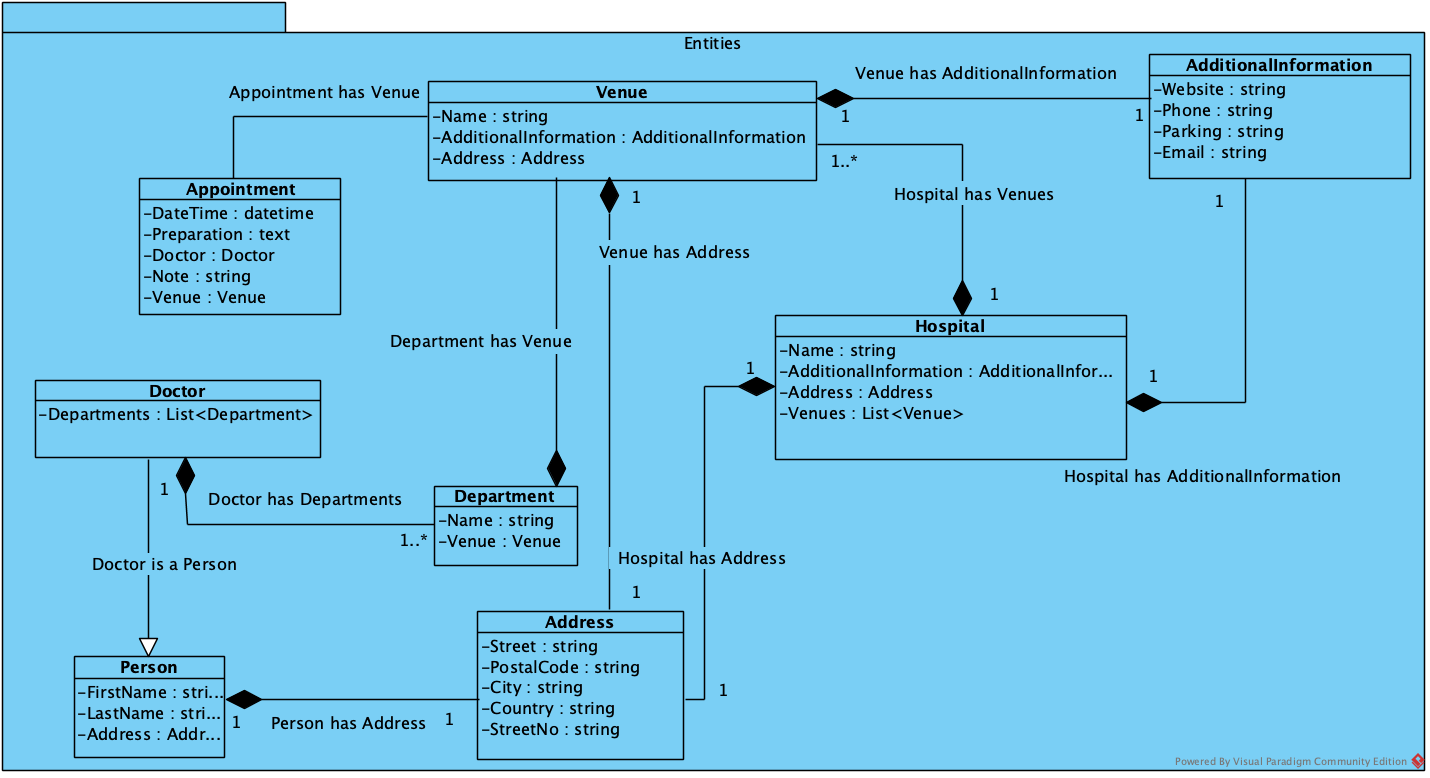
\includegraphics[scale=1]{UML_geolocalization}
\caption{Unified Modelling Language diagram}
\end{figure}
\end{landscape}
\section{Android Architecture}
\subsection{Testing}
\cite{Google_testing2017}
\begin{figure}[h!]
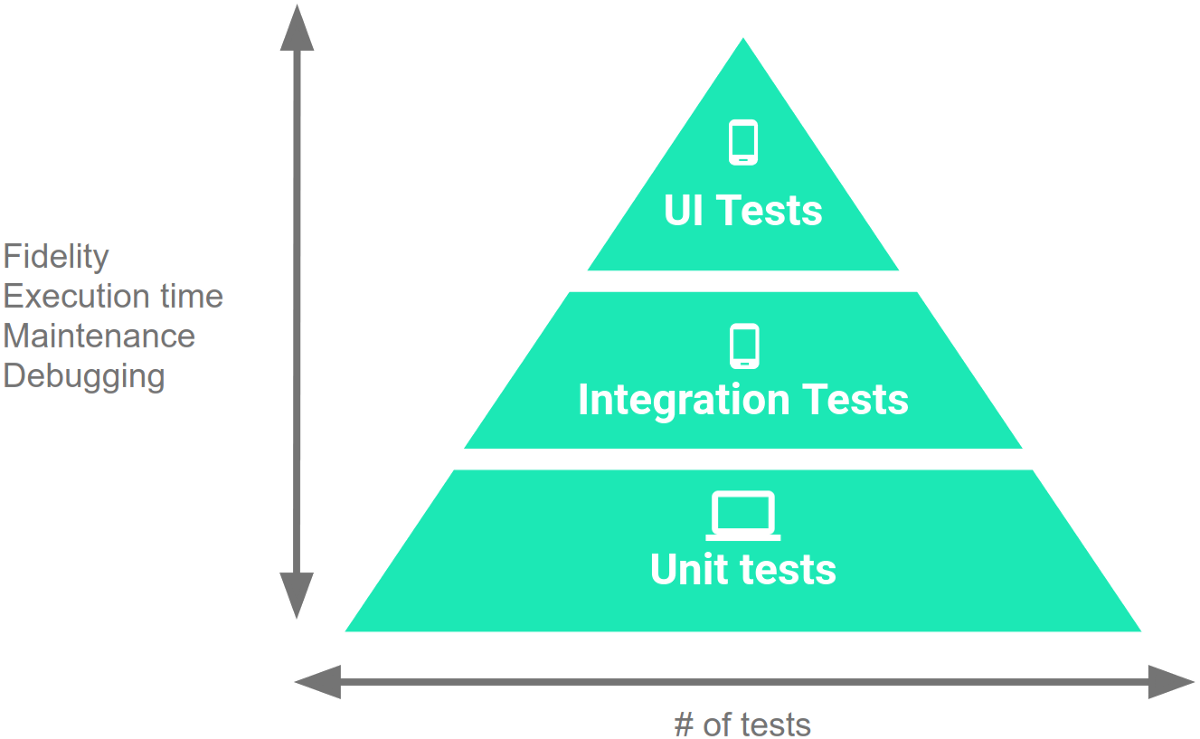
\includegraphics[scale=0.5]{testing_android}
\centering
\caption{Testing pyramid~\cite{FernandoSproviero2018}}
\end{figure}
\subsubsection{Unit Testing}
These tests are responsible for the smaller parts of the application (units) and use mocked or stubbed properties. This means that the properties and methods do not interfere with code written inside the main application. These tests are the fastest in runtime (compared to the integration and UI testing) because they do not need a running device or emulator, which means they are the least expensive to execute. Some testing frameworks from Android are: JUnit4 and Mockito (Mockito is used to create mock instances of dependencies, classes, properties and methods) \cite{FernandoSproviero2018}. The characteristics of a good unit test \cite{Google_testing2017}:
\begin{enumerate}
\item Thorough;
\item Focused;
\item Repeatable;
\item Fast;
\item Verifies behaviour;
\item Concise;
\end{enumerate}
\subsubsection{Integration Testing}
These tests test the interaction between different units of the application. The tests do not cover any updates on the UI thread and test the units independently from the UI. A common framework used to write integration tests is Roboelectric \cite{Roboelec2019}. When an application is in development the integration tests will check the behaviour of the different interacting units when the new feature is implemented. This way, the development team can roll-out features without breaking the current application.
\subsubsection{User Interface Testing}
\subsection{Separation of concern: Dependency Injection}
Separation of concern is a general convention amongst software developers. In practice it is harder to implement than it first seems. One of the core components of this pattern are dependencies: one class depends on the structure of another class. The dependency pattern enables developers to focus on their code without having to worry about the dependency. For a class it is enough to know how a dependency is structure, there is no need for the class to know how it is implemented. This is also the last of the SOLID principles, the principle of dependency on abstraction instead of concrete implementation \cite{BhavyaKaria2018}.
\subsubsection{Dependency Injection: Restaurant Analogy}
To comprehend the concept of dependency injection let's have a look at a fairly common analogy". A man comes into a restaurant and takes a look at the menu. After having taken a close look, the man decides to order fish and chips. The waiter notifies the kitchen and tells the head chef that a customer ordered the fish and chips. Upon finishing the plating, the waiter brings the wonderful plate of fish and chips to the customer (the man). The man obtained what he wanted without knowing how his dish was prepared, the head chef knew what the customer needed and provided the meal.
\subsubsection{Benefits of using Dependency Injection}
Using dependency injection might seem somewhat bloated in practice, but there are some enormous benefits upon applying this pattern on an application. Some of these benefits are listed below \cite{Seemann2011}:
\begin{itemize}
\item Late binding: interchangeable services;
\item Extensibility: reusable code;
\item Maintainability: classes with a well-defined responsibility become easier to maintain;
\item Testability: classes having a dependency can be tested separately - as a single unit; 
\item Enforces usage of loose coupling;
\end{itemize}
\subsubsection{Types of Dependency Injection}
Constructor injection is the type of DI (dependency injection) that uses a private field for the dependency and sets this field using a parameter inside of the constructor. Setter (property) injection uses a property of the class that requires the dependency and works via getter and setter methods. The dependency is individually set instead of passed as a parameter in the constructor. This is quite easy to understand but hard to implement in a robust way, this only works if the value passed in the setter is a good value. When dependencies are only used in specific methods, it might be easier to just pass them as parameters to that method, this is called method injection. This way of implementing DI is also simple and straightforward \cite{TheoJungeblut2015}.
\subsubsection{Dagger2 - Dependency Injection Library}
To remove the abstraction of the different methods of dependency injection, the library Dagger2 (supported by Google) is used. This library sets up the required dependencies throughout the application and registers them accordingly. Upon launching a class that requires a dependency, the Dagger2 instance will load them as specified in the AppModule. Since the architecture used in the application is \acrshort{mvvm}, the ViewModel is injected into an activity. The following code contains an AppModule, AppComponent, ViewModelFactoryModule and a subclass of the Application class, used for casting an activity:

\begin{verbatim}
/**
 * Component to be used to handle dependency injection
 */
@Singleton
@Component(modules = [AppModule::class, ViewModelModule::class])
interface AppComponent {
    fun inject(target: AppointmentList)
}

/**
 * Module that can be used to declare dependencies
 */
@Module
class AppModule @Inject constructor(private val app: Application) {
    @Provides
    @Singleton
    fun providesApplication(): Application {
        return app
    }

    @Provides
    @Singleton
    fun providesAppointmentViewModel(app: Application):
    AppointmentViewModel {
        return AppointmentViewModel(app, providesWebService())
    }

    @Singleton
    @Provides
    fun providesWebService(): WebService {
        return Retrofit.Builder()
            .baseUrl(Constants.BASE_URL)
            .addConverterFactory(GsonConverterFactory.create())
            .build()
            .create(WebService::class.java)
    }

    @Provides
    @Singleton
    fun providesAppointmentDao(db: AppDataBase): AppointmentDao {
        return db.appointmentDao()
    }

    @Provides
    @Singleton
    fun providesAppDatabase(app: Application): AppDataBase {
        return Room.databaseBuilder(
            app,
            AppDataBase::class.java, "app_database"
        ).fallbackToDestructiveMigration().allowMainThreadQueries().build()
    }
}


/**
 * Child Application Class to use for casting inside an activity
 * Create the AppComponent reference and uses this 
 * for injecting inside an Activity
 */
class DependencyApplication : Application() {
    lateinit var appComponent: AppComponent

    override fun onCreate() {
        super.onCreate()
        appComponent = initDagger(this)
    }

    private fun initDagger(app: DependencyApplication): AppComponent = 
    DaggerAppComponent.builder().appModule(AppModule(app)).build()

}

**
 * Factory to get the ViewModel by class for DI
 */
@Singleton
class DaggerViewModelFactory @Inject constructor(
    private val creators: Map<Class<out ViewModel>,
    @JvmSuppressWildcards Provider<ViewModel>>
) : ViewModelProvider.Factory {

    @Suppress("UNCHECKED_CAST")
    override fun <T : ViewModel> create(modelClass: Class<T>): T {
        var creator: Provider<out ViewModel>? = creators[modelClass]
        if (creator == null) {
            for ((key, value) in creators) {
                if (modelClass.isAssignableFrom(key)) {
                    creator = value
                    break
                }
            }
        }
        if (creator == null) {
            throw IllegalArgumentException("unknown model class $modelClass")
        }
        try {
            return creator.get() as T
        } catch (e: Exception) {
            throw RuntimeException(e)
        }
    }
}

@MustBeDocumented
@Target(AnnotationTarget.FUNCTION)
@Retention(AnnotationRetention.RUNTIME)
@MapKey
annotation class ViewModelKey(val value: KClass<out ViewModel>)

/**
 * Module to inject ViewModel instances
 */
@Module
abstract class ViewModelModule {

    @Binds
    abstract fun bindViewModelFactory(factory: DaggerViewModelFactory): 
    ViewModelProvider.Factory

    @Binds
    @IntoMap
    @ViewModelKey(AppointmentViewModel::class)
    abstract fun bindAppointmentsListActivity(vm: AppointmentViewModel): 
    ViewModel
}
\end{verbatim}

\subsection{Kotlin Language}
\subsection{Lifecycle Events}
For the duration of the runtime of the mobile application (from the moment the app is opened until it is closed) some events occur that are typical for an Android mobile application. A brief summary of these events is listed below (in chronological order) \cite{AndroidDeveloper2019}:
\begin{itemize}
\item onCreate() - When the activity is launched (This can happen after the onDestroy() event);
\item onStart() - When the activity is visible to the user;
\item onResume() - When the user returns to the activity after an onPause() event occurs;
\item onPause() - When activity is no longer visible;
\item onStop() - When the activity is finished or destroyed;
\item onRestart() - When the activity is restarted after a stoppage;
\item onDestroy() - When the activity is shut down;
\end{itemize}
\begin{figure}[H]
\centering
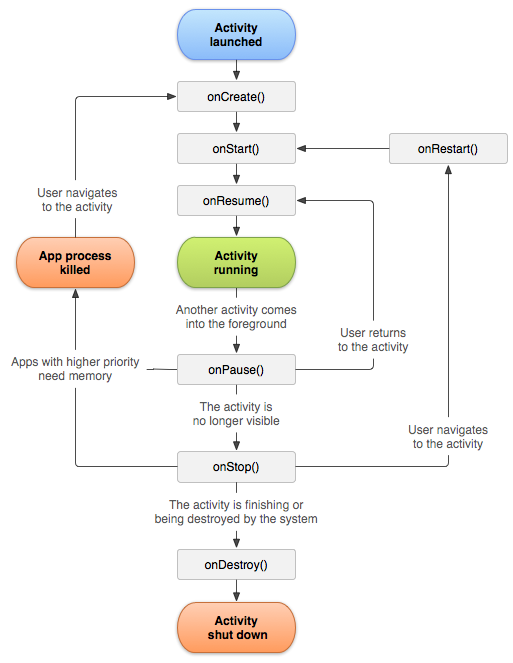
\includegraphics[scale=0.5]{activity_lifecycle}
\caption{Android Activity Lifecycle Schematic~\cite{AndroidDeveloper2019}}
\end{figure}
The lifecycle of an activity is an important factor to take into account whilst the application is being developed. This means a certain level of persistency is required for an optimal user experience.
\subsubsection{Bundles \& Saved State}
The way in which the onCreate() method is implemented allows a developer to declare a Bundle, which is an object that contains key-value pairs, that is used to restore an activity's previous state. If no such state exists then the Bundle will be equal to null. The Bundle object that is passed to an activity in the onCreate() method should only contain specific information such as user interactions: form fields, position on the screen and sometimes navigational properties. The main usage for this technology is when an activity gets paused or stopped, this means the OS (operating system) can freely destroy any activities \cite{JamesHalpern2012}.
\subsection{Offline storage and persisting data}
Another way to persist data throughout the lifecycle of an application is to use the (smart)phone's local storage. Each application can create a new local database using SQLite. SQLite is a transactional and file-based database (db), which means it is optimal for storing user-specific data. The fact that it is indeed a transactional db means that upon failure of an operation it will roll-back to the previous state and revert all existing, pending changes \cite{TutorialsPoint2019}.
\subsubsection{RoomDB}
A nice feature from the Android SDK is a wrapper for SQLite inside the app: RoomDB. RoomDB is a feature set for SQLite statement and works using the repository pattern. The interaction between the application (view layer) and data layer happens using a repository which can be implemented locally (offline storage using the RoomDB wrapper) as well as remotely (remote API calls). The structure of the application is as follows:
\begin{figure}[h!]
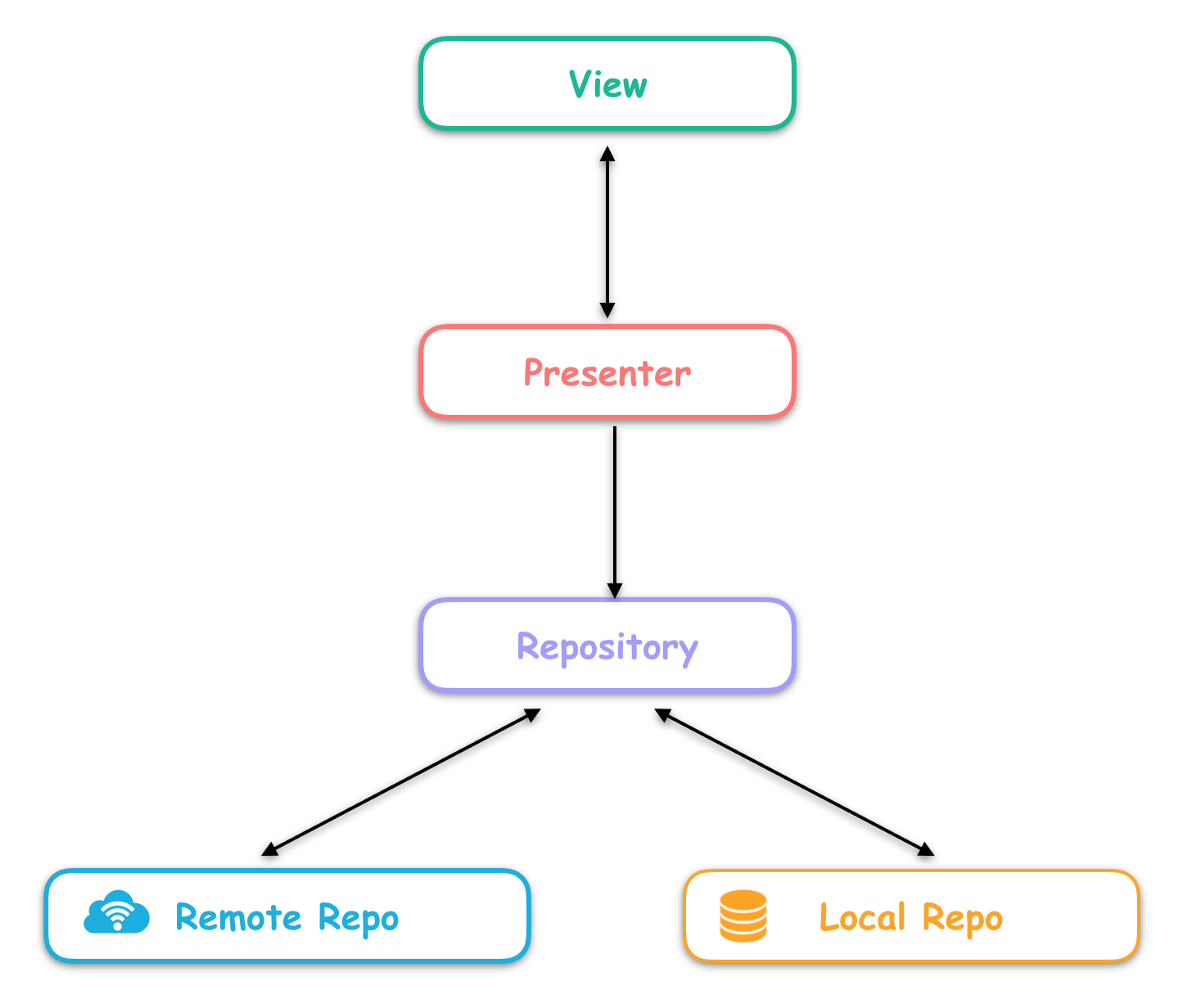
\includegraphics[scale=0.25]{repository_pattern_android}
\centering
\caption{Repository Pattern inside an android application~\cite{EslamHussein2018}}
\end{figure}
The local repository interacts with the local repository using a database access object, which specifies the different possible statements that can be executed on the database (CRUD operations: create, read, update and delete) and maps them to functions.
\begin{figure}[h!]
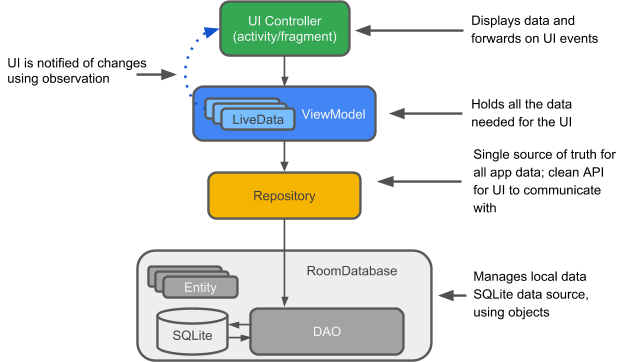
\includegraphics[scale=0.5]{local_repo_android}
\centering
\caption{Local repository usage inside the applocal~\cite{Unknown2018}}
\end{figure}

\subsubsection{Application Cache}
\subsubsection{Strategy and abstractions}
\subsection{Model - View - Presenter Architecture}
\subsubsection{Model}
\subsubsection{View}
\subsubsection{Presenter}
\subsection{Model - View - ViewModel Architecture}
\subsubsection{ViewModel}
\subsubsection{Asynchronous Data}
\subsubsection{HTTP(S) Requests}
\subsubsection{Retrofit}
\subsubsection{LiveData Datatype}
\subsubsection{Observables}